\documentclass[a4paper, 12pt]{article}
\usepackage{listings}
\usepackage{color}
\usepackage[frenchb]{babel}
\usepackage[utf8]{inputenc}
\usepackage[T1]{fontenc}
\usepackage{lmodern}
\usepackage{graphicx}
% Numbers and units
\usepackage[squaren, Gray]{SIunits}
\usepackage{sistyle}
\usepackage[autolanguage]{numprint}
\usepackage{fullpage}
\usepackage{hyperref}
\usepackage{multirow}
\usepackage{xparse}
\usepackage{tikz}
\usepackage{enumitem}
\usepackage{amsmath}

\setlength{\parskip}{1em}
\usetikzlibrary{arrows, decorations.markings}

\newcommand\si[2]{\numprint[#2]{#1}}
\newcommand\np[1]{\numprint{#1}}

\newcommand\figref[1]{figure~\ref{fig:#1}}

\NewDocumentEnvironment{myfig}{mm}
{\begin{figure}[!ht]\centering}
{\caption{#2}\label{#1}\end{figure}}

\usepackage[Conny]{fncychap}

\usepackage{enumerate}

\lstset{ %
backgroundcolor=\color{white},   % choose the background color; you must add \usepackage{color} or \usepackage{xcolor}
basicstyle=\footnotesize,        % the size of the fonts that are used for the code
breakatwhitespace=false,         % sets if automatic breaks should only happen at whitespace
breaklines=true,                 % sets automatic line breaking
captionpos=b,                    % sets the caption-position to bottom
commentstyle=\color{green},    % comment style
deletekeywords={...},            % if you want to delete keywords from the given language
escapeinside={\%*}{*)},          % if you want to add LaTeX within your code
extendedchars=true,              % lets you use non-ASCII characters; for 8-bits encodings only, does not work with UTF-8
frame=single,                    % adds a frame around the code
keywordstyle=\color{blue},       % keyword style
language=Java,                   % the language of the code
morekeywords={*,...},            % if you want to add more keywords to the set
numbers=left,                    % where to put the line-numbers; possible values are (none, left, right)
numbersep=5pt,                   % how far the line-numbers are from the code
numberstyle=\tiny\color{gray}, % the style that is used for the line-numbers
rulecolor=\color{black},         % if not set, the frame-color may be changed on line-breaks within not-black text (e.g. comments (green here))
showspaces=false,                % show spaces everywhere adding particular underscores; it overrides 'showstringspaces'
showstringspaces=false,          % underline spaces within strings only
showtabs=false,                  % show tabs within strings adding particular underscores
stepnumber=1,                    % the step between two line-numbers. If it's 1, each line will be numbered
stringstyle=\color{mauve},     % string literal style
tabsize=2,                       % sets default tabsize to 2 spaces
columns=flexible,
title=\lstname                   % show the filename of files included with \lstinputlisting; also try caption instead of title
}

\begin{document}

  \title{Formalisation du refactoring par transformations de graphe \\
  \normalsize {(Année préparatoire au Master en Sciences Informatiques, Faculte des Sciences, UMONS)}}
  \author{Paulus Alois}

  \maketitle

  \newpage

  \tableofcontents

  \newpage

  \section{Introduction}

  Qu'est ce que le refactoring ?

  Le refactoring permet de changer la structure d'un programme en vue de l'améliorer et de le clarifier tout en préservant son comportement.

  Ce procédé consiste à déplacer des méthodes, renommer des variables, supprimer des classes etc. Il est appliqué sur des programmes écrits en langage orienté objet.

  Il peut être effectué à la main par un programmeur qui va analyser le code et identifier les parties à modifier. Ensuite, celui-ci va apporter les modifications nécessaires au programme.
  Cette technique est assez lente et surtout peu sûre. En effet, le programmeur peu faire des erreurs et introduire des bugs.

  Pour pallier à cela, des outils de refactoring sont disponibles et permettent d'automatiser les actions (comme le renommage d'une variable, le déplacement d'une méthode, etc.),
  tout en garantissant une certaine sécurité par rapport au programme.

  Malheureusement, ces outils ne sont pas parfait. Ils sont pour la plupart spécialisé dans un seul language de programmation et ne garantissent pas à 100\% la préservation du comportement du programme.

  Le but de cet article sera de créer un modèle utilisable par ces outils qui sera générique et mathématiquement vérifiable.

  La structure d'un programme sera représentée sous forme de graphe et les différents refactorings par des transformations appliquées à ces graphes.
  Ce qui nous permettra de garantir la conservation de certaines propriétés du programme après un refactoring.

  Ainsi, nous aurons la possibilité de refactorer de manière automatisée sur de multiple langage de programmation tout en étant certain de conserver les fonctionnalités de notre programme.

  \newpage

  \section{Représentation en graphe}
  Pour représenter la structure d'un programme orienté objet et ses contraintes, nous aurons besoin de plusieurs types de graphes.

  \begin{itemize}[label=\textbullet]
    \item Les graphes de type
    \item Les graphes de programme
    \item Les graphes d'expression
  \end{itemize}

  En vue de pouvoir s'intégrer au mieux dans les logiciels de refactoring, la représentation en graphe s'approchera le plus possible d'un arbre de syntaxe abstrait augmenté de liens.

  Il est également important que le modèle reste concis pour faciliter sa compréhension. Seules les choses requisent pour prouver les propriétés du refactoring seront représentées.

  \subsection{Le graphe de type}

  Le graphe de type sert à spécifier les différentes contraintes qu'un graphe de programme devra respecter.
  Un graphe de programme devra respecter toutes ces contraintes ou bien être considéré comme un programme syntaxiquement incorrect.
  De ce fait, il servira à prouver que le refactoring produit des programmes valides.

  Malheureusement, le graphe de type ne suffit pas à représenter toutes les contraintes necessaires pour garantir la structure d'un programme (voir figure~\ref{contraintes}),
  il faut également y joindre un ensemble de sous-graphes interdits.

  En outre cet ensemble de sous-graphes interdits peut être infini. Par exemple l'interdiction dans une classe de contenir plusieurs variables avec le même nom,
  consiste à interdir tous les graphes contenant deux ou plusieurs variables de même nom.

  Pour régler ce problème nous aurons besoin des graphes d'expressions expliqués ci dessous.\label{subsec:grapheExpression}


  \begin{myfig}{contraintes}{Contraintes non représentables}
    \begin{enumerate}
      \item {\scriptsize une classe ne peut pas contenir plusieurs variables avec le même nom}
      \item {\scriptsize une classe ne peut pas contenir plusieurs méthodes avec la même signature}
      \item {\scriptsize une expression contenue dans une méthode ne peut pas accéder à des variables contenues dans les descendants de la classe}
      \item {\scriptsize une expression contenue dans une méthode ne peut pas accéder à un paramètre appartenent à une autre méthode.}
    \end{enumerate}
  \end{myfig}

  \subsubsection{Définition}
  Un graphe de type est un graphe étiqueté contenant un ensemble de noeuds typés et d'arêtes typées. \(G\) étant un graphe et \(TG\) un graphe typé. \(G\) est typé par rapport à \(TG\) si il existe une projection
  de \(G\) dans \(TG\) conservant les arêtes sources, les arêtes destination et les étiquettes. Pour les étiquettes, on prend en compte uniquement le nom.

  \subsubsection{Type de noeuds}

  \begin{tabular}{ | l | l | l | p{5cm} |}
    \hline
    Type & Description  \\ \hline
    C & Classe   \\ \hline
    M & Signature de méthode   \\ \hline
    MD &  Définition d'une méthode   \\ \hline
    V &  Variable   \\ \hline
    VD &  Définition d'une variable \\ \hline
    P & Paramètre \\ \hline
    E &  Expression contenue dans une définition de méthode \\ \hline
  \end{tabular}

  \subsubsection{Type d'arêtes}
  \begin{tabular}{ | l | l |  l |}
    \hline type & application & description  \\ \hline
    l : & M $\rightarrow$ MD & \\ & V $\rightarrow$ VD & lookup d'une variable ou d'une méthode à sa définition \\ \hline
    i : & C $\rightarrow$ C &  héritage d'une classe à une autre  \\ \hline
    m : & VD $\rightarrow$ C & \\ & MD $\rightarrow$ C & appartenance d'une variable ou d'une méthode à une classe  \\ \hline
    t : & V $\rightarrow$ C  & \\ &  M $\rightarrow$ C & type d'une variable ou type de retour d'un méthode   \\ \hline
    p : & MD $\rightarrow$ P  & \\ &  P $\rightarrow$ C & définition d'un paramètre ou de son type     \\ \hline
    e : & E $\rightarrow$ M & expression contenue dans une définition de méthode ou \\ & &  dans une autre expression    \\ \hline
    a : & E $\rightarrow$ {V|P} & accès à une variable ou à un paramètre    \\ \hline
    u : & E $\rightarrow$ {V|P} & mise à jour d'une variable ou d'un paramètre    \\ \hline
  \end{tabular}

  La figure~\ref{typegraphe} est un exemple de graphe de type, on peut observer toutes les relations possibles entre les noeuds typés et les arêtes typées.

  Voici quelques exemples:
  \begin{itemize}[label=\textbullet]
    \item Un noeud de type C peut hériter d'un autre noeud de type C.
    \item Un noeud de type MD contiendra des noeuds de type E et appartiendra à un noeud de type C
    \item Un noeud de type V aura comme type un noeud de type C
    \item Un noeud de type E pourra mettre à jour ou bien accèder à un noeud de type V
  \end{itemize}

  \begin{myfig}{typegraphe}{graphe de type}
    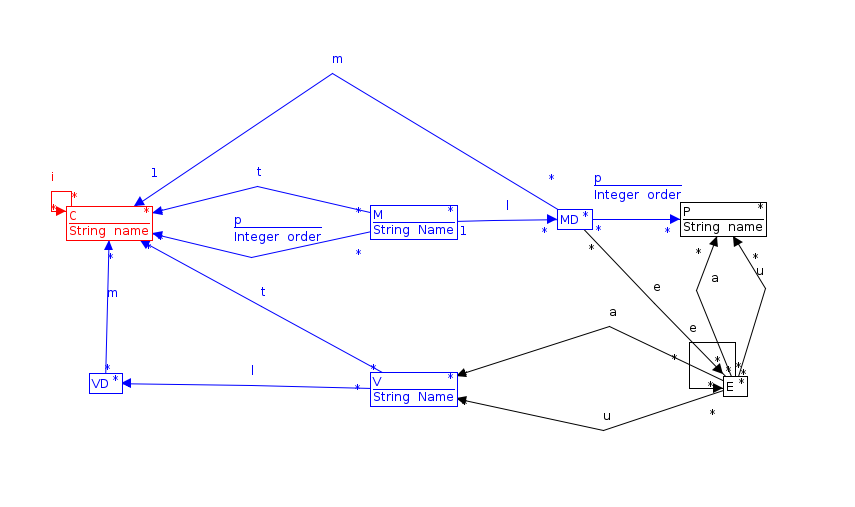
\includegraphics[width=\textwidth]{typeGraph.png}
  \end{myfig}

  \subsection{Les graphes de programme}

  Un graphe de programme est un graphe typé et étiqueté représentant la structure du code source d'un programme.
  Il est composé de noeuds typés reliés par des arêtes typées. Ses noeuds et ses arêtes prennent les valeurs vues dans le graphe de type figure~\ref{typegraphe}
  et sont agrémentés d'un nom et/ou d'autres attributs. La figure~\ref{typedgraphe} est un exemple de graphe de programme.

  \subsubsection{Definition}
  \(G \) est composé d'un ensemble de noeuds étiquetés et d'arêtes étiquetées, c'est un graphe formé de triplet, ({$V_G$},{$E_G$},\(nlabg \)), où {$V_G$} est un ensemble de noeuds,
  \(nlabg \) est une fonction d'étiquetage de noeud et {$E_G$} est un ensemble d'arêtes. Les arêtes sont représentées par un triplet (noeud départ, étiquette, noeud destination).

  Dans un graphe de programme les entités (classes, variables, méthodes et paramètres) sont représentées par des noeuds dont l'étiquette est une paire composée d'un nom et d'un type.
  Et les relations entre ces différentes entités (héritage, appel de méthodes, appartenance) sont représentées par des arêtes.

  Ces arêtes possèdent une étiquette afin de faire la différence entre les arêtes de même type ayant le même noeud source et le même noeud destination.

  \begin{myfig}{typedgraphe}{graphe de programme}
    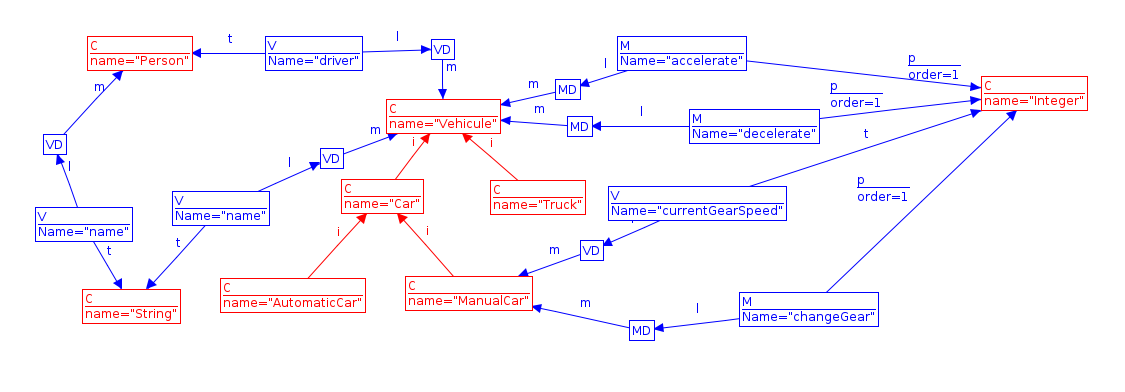
\includegraphics[width=\textwidth]{typedGraph.png}
  \end{myfig}

  \subsection{Les graphes d'expression}

  Dans la section~\ref{subsec:grapheExpression} nous avons évoqué les graphes d'expressions en vue de représenter des contraintes supplémentaires.

  Ces graphes possèdent des arêtes dont les étiquettes peuvent être des expressions régulières, ceci permet de représenter un ensemble de graphe à partir d'un seul graphe.

  Il suffit de remplacer les expressions régulières par leurs valeurs et de créer un graphe pour chacune de celle-çi, Comme sur l'exemple de la figure~\ref{grapheExpression}

  \begin{myfig}{grapheExpression}{graphe d'expression}
    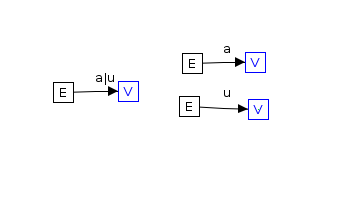
\includegraphics{graphExpression.png}
  \end{myfig}

  Sur la gauche de la figure~\ref{grapheExpression} se trouve un graphe avec une arête dont l'étiquette est une expression régulière.

  A droite, sont représentés les deux graphes issus du premier graphe, une expression mettant à jour une variable et une expression accédant à une variable.

  L'exemple reste assez simple mais vous pouvez imaginer un graphe qui peut representer des centaines d'autres graphes.

  \section{Cas d'étude}

  Dans ce rapport, nous étudierons deux refactoring en particulier.

  \begin{enumerate}
    \item PullUpMethod qui consiste à supprimer une méthode présente dans une ou plusieur classes enfant et à l'insérer dans la classe parent.
    \item EncapsulateVariable qui consiste à imposer l'accès et la mise à jour d'une variable par l'intermédiaire de deux méthodes communément appelées getter et setter.
  \end{enumerate}

  Les exemples seront pris sur base du programme Transport, c'est un programme simple écrit en java permettant ces deux refactorings.

  Certains exemples donnés sous forme de graphe ont été réalisés à l'aide de l'outil AGG.

  Les caractéristiques de AGG sont:

  \begin{itemize}[label=\textbullet]
    \item Représenter des structures de données sous forme de graphe qui peuvent être typé par un graphe de type.
    \item Spécifier des contraintes sur un graphe
    \item Spécifier des NAC pour exprimer des conditions de non-existance de certaines structures lors de transformation de graphe.
    \item Application de transformation de graphe
    \item Application séquentielle de transformation de graphe
  \end{itemize}

  AGG est assez facile à prendre en main, surtout grâce aux exemples fournis. Cet outil m'a aidé à comprendre certains concepts comme les NACs et m'a été très utile durant toute la rédaction de ce rapport.

  \subsection{Code source du programme Transport}

  \begin{lstlisting}[frame=single]
    public class Vehicule {
    public String name;
    public Person driver;

    public void accelerating(int amount) {

    }

    public void decelerate(int amount) {

    }
    }

    public class Truck extends Vehicule {

    }

    public class Person {
    public String name;
    }

    public class ManualCar {
    public int currentGearSpeed;

    public void changeGear(int number) {
    }
    }

    public class Car extends Vehicule {

    }

    public class AutomaticCar {

    }
  \end{lstlisting}

  \newpage
  \section{Refactoring}

  \subsection{Préservation du comportement}
  \label{subsec:preservationDuComportement}

  La conservation du comportement d'un programme est primordiale lors d'un refactoring.
  Malheureusement, il n'est pas facile de définir en quoi consiste réellement cette préservation.

  Par ailleurs, il sera nécessaire de trouver une définition suffisante garantissant que le programme effectuera les mêmes actions avant et après le refactoring.

  Dans cette optique, nous nous concentrerons ici sur trois propriétés.

  \begin{itemize}[label=\textbullet]
    \item Préservation de l'accès, chaque méthode accédera au moins à toutes les variables auxquelles elle accédait avant le refactoring
    \item Préservation de la mise à jour, chaque méthode mettra à jour au moins toutes les variables qu'elle mettait à jour avant le refactoring
    \item Préservation de l'appel, chaque méthode appellera au moins toutes les méthodes qu'elle appelait avant le refactoring
  \end{itemize}

  \subsection{Transformation de graphe}

  Pour représenter un refactoring appliqué sur le code source d'un programme, on applique des transformations de graphe sur le graphe de programme.

  Il reste cependant quelques problèmes:

  \begin{enumerate}
    \item Certains types de refactoring modifient une partie variable d'un programme, ce qui les rend impossible à représenter grâce à une simple transformation.
    Il faut donc appliquer plusieurs transformations l'une après l'autre dans un ordre spécifique. Pour cela nous aurons besoin d'un mécanisme de réécriture de graphe.

    \item Un refactoring devra être défini sous forme générique et non spécifique aux noms des classes/méthodes contenues dans le programme sur lequel ce refactoring est appliqué.
    Pour cela, une technique de production de graphe avec paramètre va être employée.

    \item Il est possible que certaines arêtes ne pointent plus vers un noeud suite a l'application d'un refactoring.
    Par exemple, si elles accédaient à une variable qui est maintenant uniquement accessible par des méthodes (getter ou setter).
    Ces arêtes ne sont normalement pas autorisées mais les éviter serait trop complexe car nous aurions besoin de créer des ensembles LHS et RHS infinits.
    Pour pallier à ce problème, on emploie un mécanisme appelé ``embedding mechanism'' qui autorise ces arêtes orphelines et qui précisera comment les rediriger vers un autre noeud.
  \end{enumerate}

  \subsubsection{Règles de transformation}

  Quelques notions doivent être définies avant de pouvoir appliquer une production à un graphee:

  \begin{enumerate}
    \item \(G\) étant un graphe, un sous graphe de \(G\) contient un ensemble de noeuds de \(G\) et uniquement les arêtes reliant les noeuds contenus dans ce sous graphe.

    \item Lorsque l'on applique un mappage sur les noeuds de \(G\), on applique automatiquement un mappage sur les arêtes reliant ces noeuds.

    \item \(G\) et \(K\) étant des graphes, une occurrence de \(K\) dans \(G\) nécessite que toutes les arêtes entre les noeuds correspondants existent.

  \end{enumerate}

  \tikzstyle{weight} = [font=\small]
  \tikzstyle{edge} = [draw,line width=2pt,-,black]
  \tikzstyle{vertex}=[circle,fill=black!25,minimum size=10pt,inner sep=0pt]
  \begin{myfig}{sousgraphe1}{graphe}
    \begin{tikzpicture}[scale=1.8, auto,swap]

      % First we draw the vertices
      \foreach \pos/\name in {{(0,2)/b}, {(2,2)/c}, {(1,1)/e},
      {(0,0)/a}, {(2,0)/d}}
      \node[vertex] (\name) at \pos {$\name$};
      % Connect vertices with edges and draw weights
      \foreach \source/ \dest /\weight in {a/b/1, c/b/2,c/d/3,d/a/4,
      e/c/5, b/e/6}
      \path[edge] (\source) -- node[weight] {$\weight$} (\dest);

    \end{tikzpicture}
  \end{myfig}


  \begin{myfig}{sousgraphe2}{Exemple sous graphe valide / invalide}
    \tikzstyle{edge} = [draw,line width=2pt,-,green]
    \tikzstyle{vertex}=[circle,fill=green!25,minimum size=10pt,inner sep=0pt]
    \begin{tikzpicture}[scale=1.8, auto,swap]

      % First we draw the vertices
      \foreach \pos/\name in {{(0,2)/b}, {(2,2)/c}, {(1,1)/e}}
      \node[vertex] (\name) at \pos {$\name$};
      % Connect vertices with edges and draw weights
      \foreach \source/ \dest /\weight in {c/b/2,
      e/c/5, b/e/6}
      \path[edge] (\source) -- node[weight] {$\weight$} (\dest);

      \tikzstyle{edge} = [draw,line width=2pt,-,red]
      \tikzstyle{vertex}=[circle,fill=red!25,minimum size=10pt,inner sep=0pt]

      % First we draw the vertices
      \foreach \pos/\name in {{(3,2)/b}, {(5,2)/c}, {(4,1)/e}}
      \node[vertex] (\name) at \pos {$\name$};
      % Connect vertices with edges and draw weights
      \foreach \source/ \dest /\weight in {c/b/2, b/e/6}
      \path[edge] (\source) -- node[weight] {$\weight$} (\dest);
    \end{tikzpicture}
  \end{myfig}

  \subsubsection{Définition}

  La définition mathématique est donnée dans l'article~\cite[p.~15]{mainArticle}.

  Je vais tout de même l'expliquer à l'aide des figures~\ref{sousgraphe1} et \ref{sousgraphe2}.

  \(G\) et \(H\) sont des graphes, \(m\) est une fonction de mappage de \(L\) vers \(G\) et \(n\) est une fonction de mappage de \(R\)  vers \(H\) .

  \(m(v)\) est un sous graphe de \(G\) et \(n(w)\) est un sous graphe de H.

  $V_H$ est égal au graphe \(({V_G} \setminus m({V_L})) \cup n({V_R})\). De facon très imagée on peut voir ça comme un oeuf dont on retirerait le jaune d'oeuf et on le remplacerait par un autre.

  La fonction $Emb_{in}$ est utilisée pour rediriger les arêtes partant de noeuds contenus dans \( {V_G}~\setminus~m({V_L}) \)
  qui pointaient vers des noeuds contenus dans \( m({V_L}) \) à des arêtes d'un noeuds de \( {V_H} \setminus n({V_R}) \) à un noeuds de \( n({V_R}) \).

  La fonction $Emb_{out}$ est utilisée pour rediriger les arêtes partant de noeuds contenus dans \( m({V_L}) \)
  qui pointaient vers des noeuds de \( {V_G}~\setminus~m({V_L}) \) à des noeuds de \(n({V_R}) \) vers des noeuds de \( {V_H}~\setminus~n({V_R}) \).

  \begin{myfig}{sousgraphe}{$Emb_{out}$ et $Emb_{out}$}
    \tikzset{>=latex}
    \begin{tikzpicture}
      \node[] at (1,5) {L};
      \draw (2,4) ellipse (1cm and 0.5cm);
      \node[] at (2,4) {V};

      \draw[->] (5,4) -- +(1,0);
      \draw[->] (2,3) -- +(0,-1) node[anchor=west] {m};

      \node[] at (8,5) {R};
      \draw (9,4) ellipse (1cm and 0.5cm);
      \node[] at (9,4) {W};

      \draw[->] (9,3) -- +(0,-1) node[anchor=west] {n};

      \node[] at (0,1) {G};
      \draw (2,0) ellipse (2cm and 1cm);
      \draw (2,0) ellipse (1cm and 0.5cm);
      \node[] at (2,0) {m(v)};

      \draw[->] (5,0) -- +(1,0);

      \draw (3.5,0) node[anchor=south] (e) {\textbullet};
      \draw (2.5,0) node[anchor=south] (f) {\textbullet};

      \draw (0.5,0) node[anchor=south] (g) {\textbullet};
      \draw (1.5,0) node[anchor=south] (h) {\textbullet};

      \draw[-latex] (e.west) to[out=90,in=70] (f.east);

      \draw[-latex] (h.west) to[out=70,in=90] (g.east);

      \node[] at (7,1) {H};
      \draw (9,0) ellipse (2cm and 1cm);
      \draw (9,0) ellipse (1cm and 0.5cm);
      \node[] at (9,0) {n(w)};

      \draw (10.5,0) node[anchor=south] (a) {\textbullet};
      \draw (9.5,0) node[anchor=south] (b) {\textbullet};

      \draw (7.5,0) node[anchor=south] (c) {\textbullet};
      \draw (8.5,0) node[anchor=south] (d) {\textbullet};

      \draw[-latex] (a.west) to[out=90,in=70] (b.east);

      \draw[-latex] (d.west) to[out=70,in=90] (c.east);

    \end{tikzpicture}

  \end{myfig}


  \begin{myfig}{LHSRHSPullUpMethod}{LHS et RHS}
    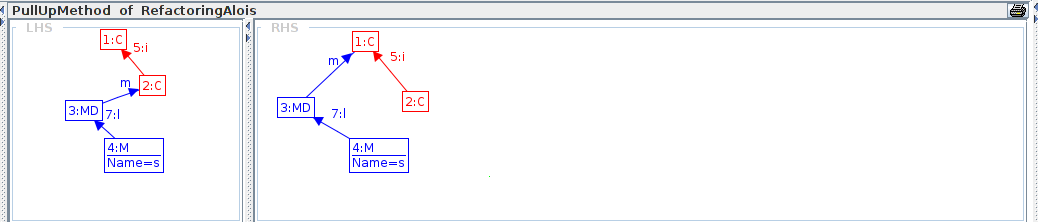
\includegraphics[width=\textwidth]{LHSRHSPullUpMethod.png}
  \end{myfig}

  \subsection{Précondition de refactoring}
  Les préconditions servent à définir un sous graphe ou un ensemble de sous graphe ne pouvant pas être présent avant d'appliquer le refactoring.
  Nous pourrions également employer des postconditions pour interdire certains sous graphes dans le graphe résultat
  mais les préconditions sont plus adaptées car on évite d'appliquer des transformations sur un graphe et ensuite seulement de détecter les erreurs.

  \begin{myfig}{NACPullUpMethod}{NAC}
    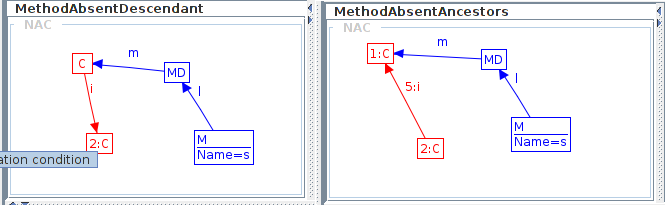
\includegraphics[width=\textwidth]{NACPullUpMethod.png}
  \end{myfig}

  La figure~\ref{NACPullUpMethod}, représente les deux préconditions nécessaires pour pouvoir appliquer le refactoring PullUpMethod.
  Elle spécifie qu'aucun ancêtre ni descendant de la classe ne peut posséder cette méthode avant le refactoring.


  \section{Application sur le programme transport}

  \subsection{Encapsulate Variable}

  Encapsuler une variable dans une classe est une opération souvent éffectué par les programmeurs.
  Elle consiste à transformer une variable publique en variable privée.
  Et à ajouter un accesseur public et un setter public pour continuer à accéder et à mettre à jour cette variable.

  Lors d'un refactoring cela consiste à changer la visibilité de la variable et à créer deux nouvelles méthodes.
  Ensuite, il faut changer tous les accès ou/et mises à jour de la variable par des appels aux deux méthodes créées.

  \subsubsection{Conditions}

  \begin{itemize}[label=\textbullet]
    \item Les deux nouvelles méthodes créées ne sont pas déjà présentes dans la classe
    \item Les deux nouvelles méthodes créées ne sont pas déjà présentes dans ses ancêtres
    \item Les deux nouvelles méthodes créées ne sont pas déjà présentes dans ses descendants.
  \end{itemize}

  \subsubsection{Contraintes}

  Les contraintes de la figure~\ref{contraintes} sont préservées:
  \begin{enumerate}
    \item est préservée car on ne crée ni ne déplace aucune variable.
    \item est préservée car la condition stipule qu'il ne faut pas que des méthodes comportant les mêmes définitions que le getter ou le setter soient présentes.
    \item est préservée car on crée deux méthodes accédant à une variable dans la même classe.
    \item est préservée car le paramètre de la méthode setter est employée uniquement dans la définition de cette méthode.
  \end{enumerate}

  \subsubsection{Code source avant le refactoring}

  \begin{lstlisting}[frame=single]
    public class Person {
    public String name;
    }
  \end{lstlisting}

  \subsubsection{Code source après le refactoring}

  \begin{lstlisting}[frame=single]
    public class Person {
    private String name;

    public String GetName(){
    return name;
    }

    public void SetName(String n){
    name=n;
    }
    }
  \end{lstlisting}

  \subsubsection{Représentation graphique}

  \begin{myfig}{beforeEncapsulateVariable}{Before Encapsulate Variable}
    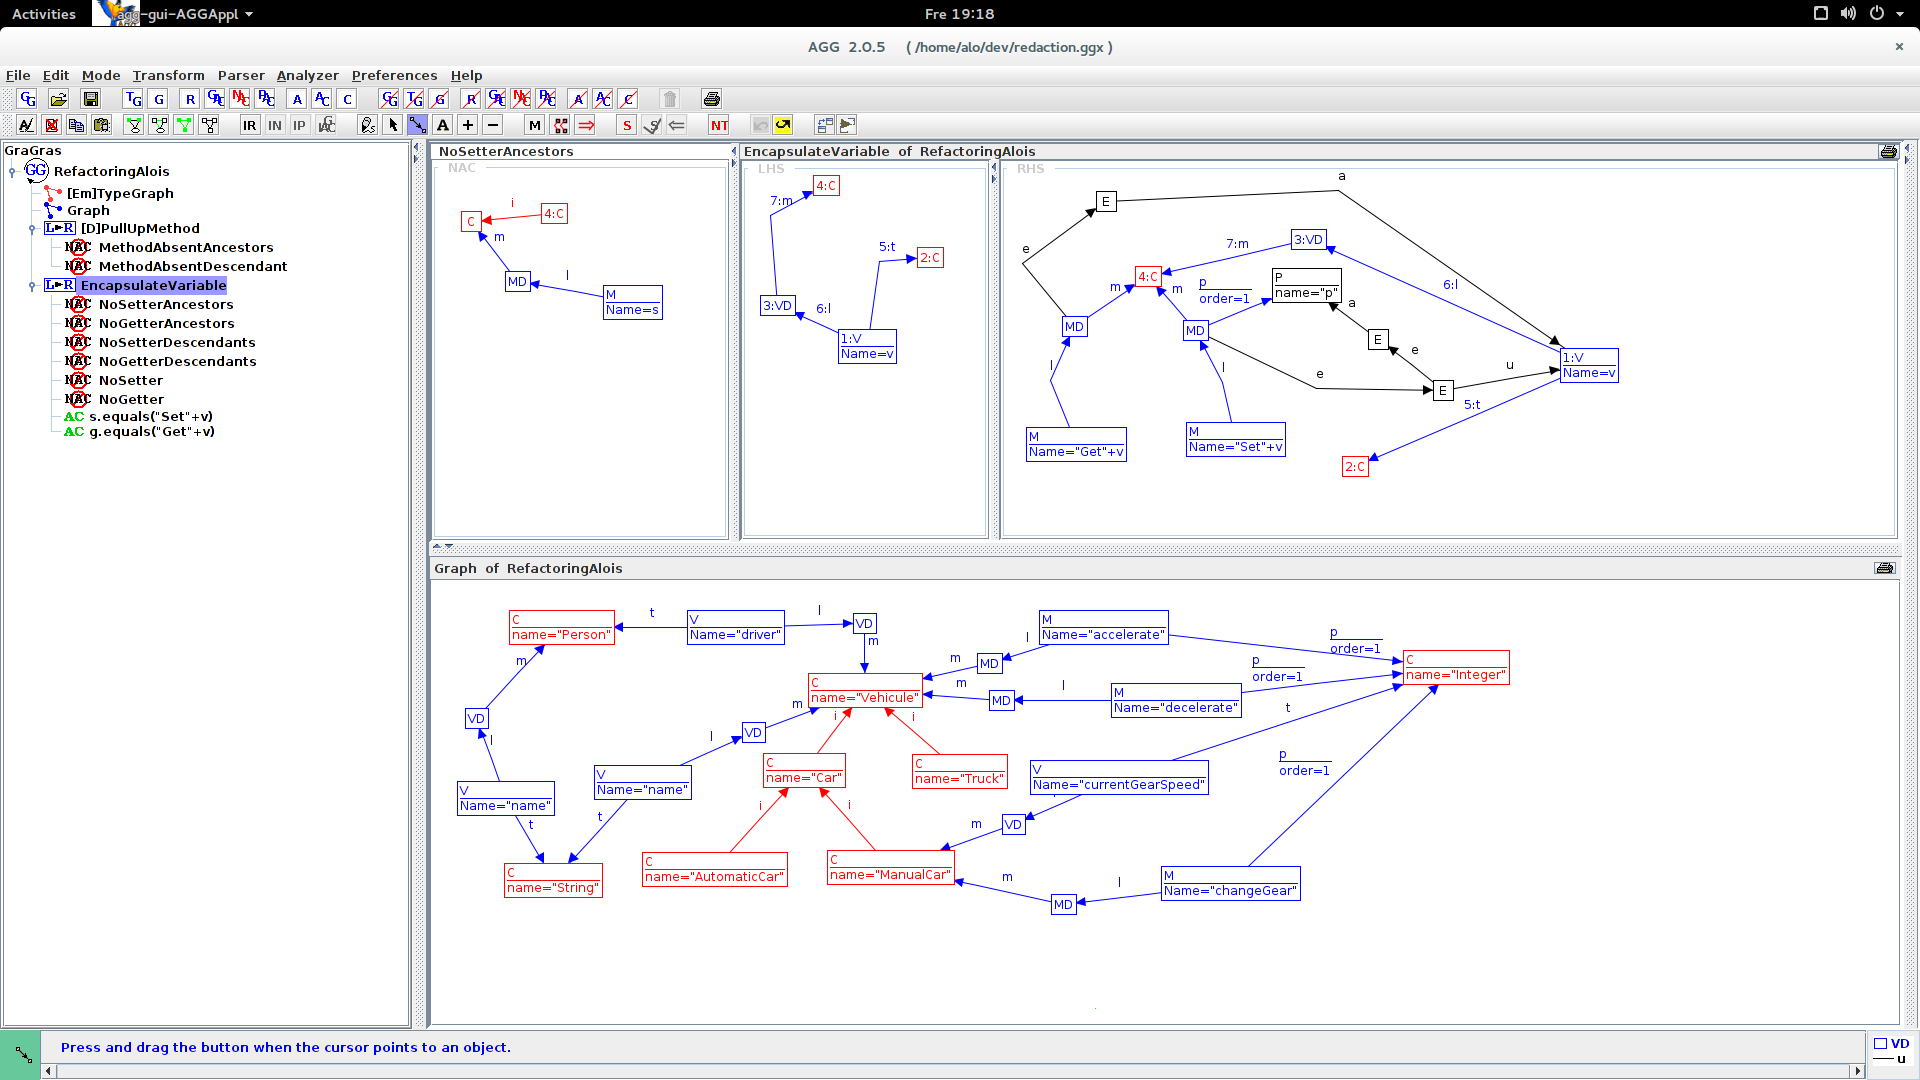
\includegraphics[width=\textwidth]{beforeEncapsulateVariable.png}
  \end{myfig}

  Dans le haut de la figure~\ref{beforeEncapsulateVariable} se trouve la LHS qui représente le sous graphe du programme à transformer.
  A droite, nous avons RHS qui représente la structure de ce sous graphe après la transformation.
  Et en dessous nous avons le graphique du programme.

  \begin{myfig}{afterEncapsulateVariable}{After Encapsulate Variable}
    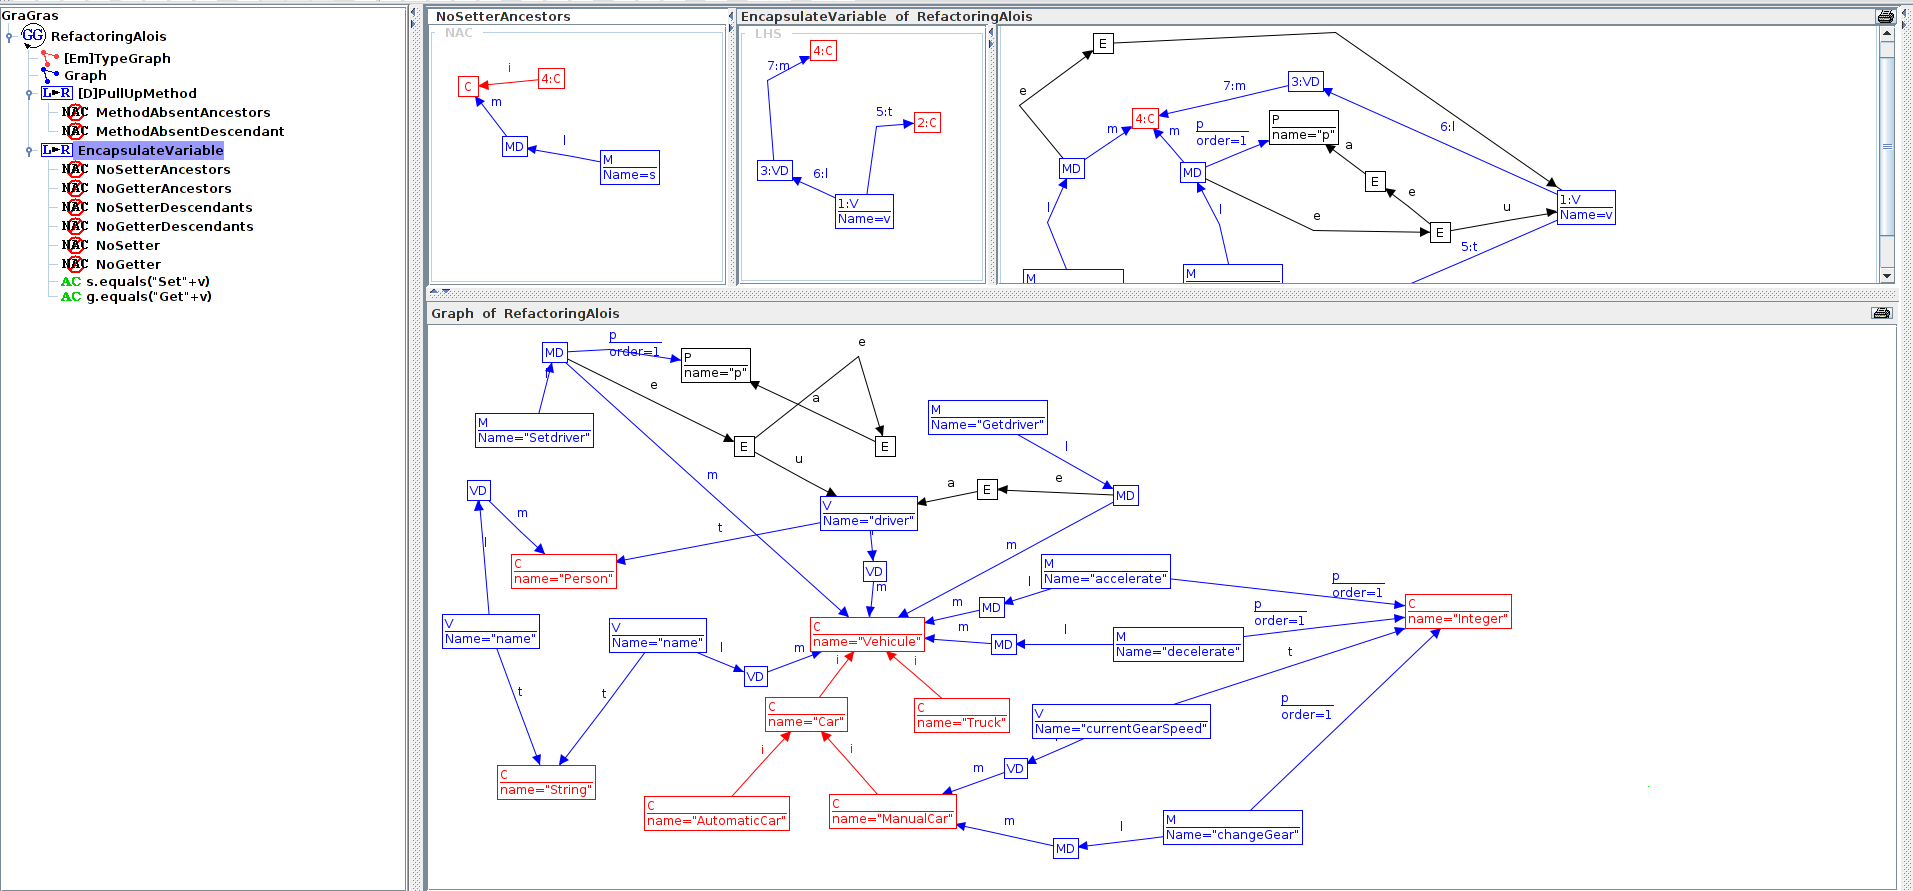
\includegraphics[width=\textwidth]{afterEncapsulateVariable.png}
  \end{myfig}

  Dans la figure~\ref{afterEncapsulateVariable}, la partie inférieure a changé.
  Elle représente le grapheique après l'application de la/les transformation(s). On peut voir que de nouveaux noeuds et de nouvelles arêtes ont été créés pour représenter les deux nouvelles méthodes.

  Je n'ai laissé que la transformation du sous graphe lié à la variable ``driver'' pour une meilleure visibilité.

\clearpage

  \subsection{Pull Up Method}

  Cela consiste à déplacer une méthode présente dans une ou plusieurs classes enfant dans leur classe parent.

  \subsubsection{Conditions}

  \begin{itemize}[label=\textbullet]
    \item La classe parent ne peut pas déjà contenir une méthode ayant la même signature
    \item Aucune des variables directement accédée ou modifiée par la méthode ne peut être en dehors de la portée (scope) de la classe parent.
  \end{itemize}

  \subsubsection{Contraintes}

  Les contraintes de la figure~\ref{contraintes} sont préservées:
  \begin{enumerate}
    \item est préservée car on ne crée ni ne déplace aucune variable.
    \item est préservée grâce à la précondition qui stipule qu'il ne peut pas se trouver une méthode avec la même signature dans la classe parent.
    \item est préservée grâce à la précondition qui stipule que la définition de la méthode déplacée ne doit pas accéder à des variables en dehors du scope du parent.
    \item est préservée car on ne crée ni ne modifie aucune méthode.
  \end{enumerate}

  \subsubsection{Code source avant le refactoring}
  \begin{lstlisting}[frame=single]
    public class Vehicule {
    public String name;
    public Person driver;

    public void accelerating(int amount) {
    }

    public void decelerate(int amount) {
    }
    }

    public class Car extends Vehicule {

    }

    public class ManualCar extends Car {
    public void changeGear(int speed){
    }
    }
  \end{lstlisting}

  \subsubsection{Code source après le refactoring}
  \begin{lstlisting}[frame=single]
    public class Vehicule {
    public String name;
    public Person driver;

    public void accelerating(int amount) {

    }
    public void decelerate(int amount) {
    }

    public void changeGear(int speed){
    }
    }

    public class Car extends Vehicule {

    }

    public class ManualCar extends Car {

    }
  \end{lstlisting}

  \subsubsection{Représentation graphique}

  \begin{myfig}{beforePullUpMethode}{Before PullUp Methode}
    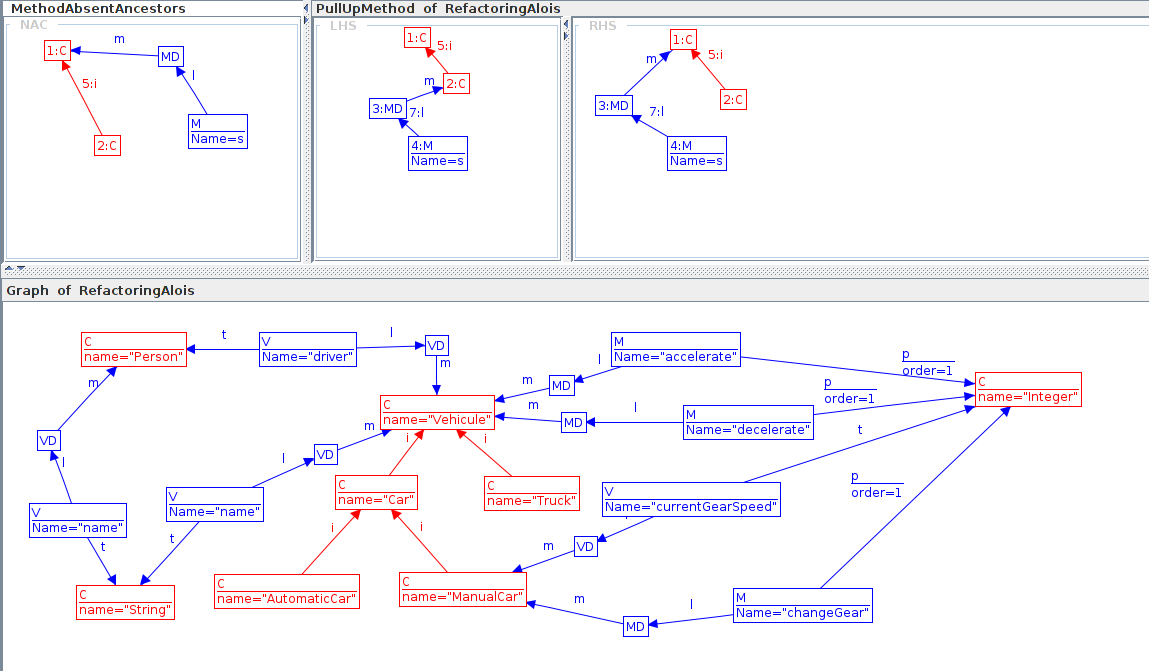
\includegraphics[width=\textwidth]{beforePullUpMethode.png}
  \end{myfig}

  En haut à gauche de la figure~\ref{beforePullUpMethode} se trouve la LHS qui représente la structure du sous graphe à transformer.
  En haut à droite de la figure~\ref{beforePullUpMethode} se trouve la RHS qui représente la structure de ce sous graphe après la transformation.
  En dessous, nous avons le grapheique du programme.

  \begin{myfig}{afterPullUpMethod}{After PullUp Methode}
    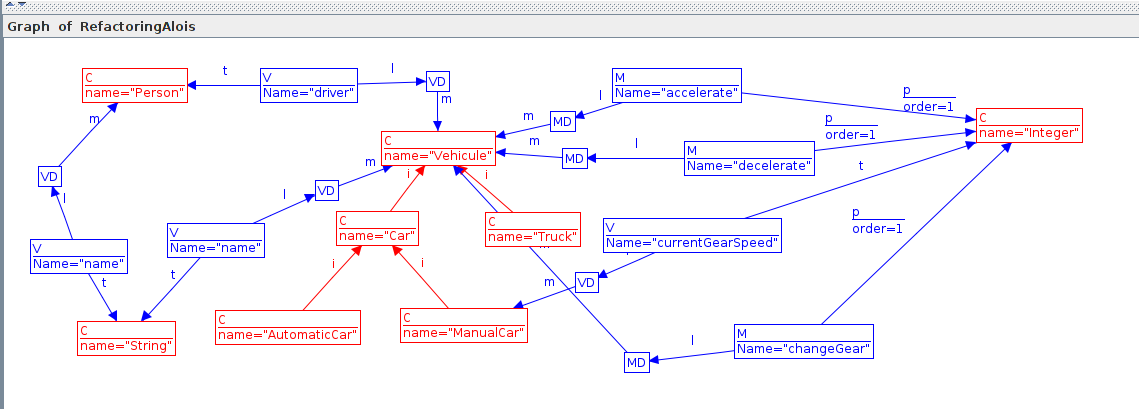
\includegraphics[width=\textwidth]{afterPullUpMethod.png}
  \end{myfig}

  Dans la figure~\ref{afterPullUpMethod} la partie du dessous a changé et représente le programme après avoir appliqué la transformation.
  Après avoir remonté la méthode de la classe ManualCar dans la classe Vehicule,
  on peut observer que le lien de la méthode ``changeGear'' vers la classe ManualCar n'existe plus. Et qu'un nouveau lien a été créé vers la classe Vehicule.

  \section{Préservation du comportement du programme}

  Jusqu'ici nous avons défini des mécanismes permettant de refactorer un programme à l'aide de graphe. Il nous reste encore à prouver que ce programme conserve son comportement à la suite de ces transformations.

  Le but de cette partie est donc de démontrer que certaines propriétés du programme sont préservées après un refactoring:
  \begin{itemize}[label=\textbullet]
    \item l'accès aux variables
    \item la mise à jour de variables
    \item l'appel de méthode
  \end{itemize}

  Pour cela, nous avons besoin d'introduire le concept d'une fonction de tracking appelée, \(tr\).

  \subsection{Définition, préservation d'une expression de graphe}

  \(GE\) étant un graphe d'expression, \(G\) et \(H\) étant des graphes de programme. La fonction \(tr: {V_G} \rightarrow {V_H}\)
  est un mappage de noeuds tels que pour chaque occurrence \( oc \) de $GE$ dans $G$, la composition de fonction  \(tr \circ oc \) est une occurrence de $GE$ dans $H$.

  Pour chaque production de graphe, une fonction $tr$ existe et mappe les noeuds de LHS dans ceux de RHS.

  \subsection{Fonction de tracking}

  \subsubsection{Définition}
  Si \(G\) derive \(H\) grâce à une production \( P = (L,R,Emb_{in} ,Emb_{out} ) \) via $m$ et $n$, alors la fonction de tracking $tr : {V_G} \rightarrow {V_H} $ est définie comme suit :
  \[ tr(v) =
  \begin{cases}
    n \circ trp \circ m^{-1}(v) & \text{si }v\text{ est une node de }m(L)\\
    v & \text{si }v\text{ n'est pas une node de }m(L)
  \end{cases}
  \]

  Cette définition mathématique définit :
  \begin{itemize}[label=\textbullet]
    \item Pour tous noeuds contenus dans \( {V_L} \) , la fonction \(m^{-1}(v)\) va chercher le noeud dans {$V_G$} et le mappe dans \( L \). Ensuite la fonction de tracking mappe le noeud de  \( L \)
    dans  $R$  et enfin la fonction \( n \) mappe le noeud de  \( R \)  dans {$V_H$}.
    \item Pour tous les autres noeuds, aucune manipulation particulière n'est requise.
  \end{itemize}

  \subsection{Préservation du comportement : Encapsulate Variable}

  \subsubsection{Production}

  \begin{myfig}{embedding}{méchanisme ``embedding''}
    \begin{center}
      \begin{tikzpicture}[->,>=stealth',shorten >=1pt,auto,node distance=3cm,
        thick, label distance=-1mm, label position=45, every label/.style={red}]

        \node [draw,thick,minimum width=1cm,minimum height=0.5cm,label=1] at (0,1)  (varLeft) {var V};

        \draw[thick,->] (1,1) -- (3,1);
        \node[red] at (2,0.5) {P1};

        \node (rect) at (4,2) [draw,thick,minimum width=1cm,minimum height=0.5cm,label=3] (setter) {Setter M};
        \node (rect) at (4,0) [draw,thick,minimum width=1cm,minimum height=0.5cm,label=4] (getter) {Getter M};
        \node (rect) at (6,1) [draw,thick,minimum width=1cm,minimum height=0.5cm,label=1] (varRight) {var V};

      \end{tikzpicture}
    \end{center}

    \begin{center}
      \begin{tikzpicture}[->,>=stealth',shorten >=1pt,auto,node distance=3cm,
        thick, label distance=-1mm, label position=45, every label/.style={red}]
        \tikzstyle{EdgeStyle}=[bend left]

        \node at (0,2) ["180:$2$", draw,thick, minimum width=1cm, minimum height=0.5cm] (setter) {Setter M};
        \node at (0,0) [draw,thick,minimum width=1cm,minimum height=0.5cm,label=3] (getter) {Getter M};
        \node at (3,2) [draw,thick,minimum width=1cm,minimum height=0.5cm,label=1] (varLeft) {var V};
        \node (rect) at (3,0) [draw,thick,minimum width=1cm,minimum height=0.5cm] (vdLeft) {VD};

        \draw[thick,->] (4,1) -- (6,1);
        \node[red] at (5,0.5) {P2};

        \node at (7,2) [draw,thick,minimum width=1cm,minimum height=0.5cm,label=4] (mdSetter) {MD};
        \node at (7,0) [draw,thick,minimum width=1cm,minimum height=0.5cm,label=2] (setter) {Setter M};
        \node at (9.5,2) [draw,thick,minimum width=1cm,minimum height=0.5cm,label=1] (varRight) {var V};
        \node at (9.5,0) [draw,thick,minimum width=1cm,minimum height=0.5cm,label=0] (vdRight) {VD};
        \node at (12,2) [draw,thick,minimum width=1cm,minimum height=0.5cm,label=5] (mdGetter) {MD};
        \node at (12,0) [draw,thick,minimum width=1cm,minimum height=0.5cm,label=3] (getter) {Getter M};

        \path[every node/.style={font=\sffamily\small}]
        (setter) edge [left] node [right] {l} (mdSetter)
        (getter) edge [left] node [right] {l} (mdGetter)
        (mdGetter) edge node {a} (varRight)
        (mdSetter) edge node {u} (varRight)
        (varLeft) edge [left] node [right] {l} (vdLeft)
        (varRight) edge [left] node [right] {l} (vdRight);
      \end{tikzpicture}
    \end{center}


    \begin{tabular}{ | l | l |  l |}
      \hline production & arêtes entrantes & arêtes sortantes  \\ \hline
      P1 : & (\(a,1) {\rightarrow} (a,1)\) &  (\(t,1) {\rightarrow}(t,1),(1.p,2),(t,3)\)   \\ \hline
      & (\(u,1) {\rightarrow} (u,1)\) & \( (l,1) {\rightarrow} (l,1)\)  \\ \hline
      P2 : & \((a,1) {\rightarrow} (c,3)\) &  \((m,0) {\rightarrow} ((m,0),(m,4),(m,5)\)    \\ \hline
      & (\(u,1) {\rightarrow} (c,2)\) &  \((t,1) {\rightarrow} (t,1)\)  \\ \hline
    \end{tabular}
  \end{myfig}

  Sur la figure~\ref{embedding} on peut faire différentes observations grâce aux graphes et égalemment à la table :

  \begin{itemize}[label=\textbullet]
    \item Les noeuds ayant les mêmes numéros sont des noeuds conservés entre les productions.
    \item Le type de la variable reste inchangé
    \item Le type de retour du getter est identique à celui de la variable
    \item Le type du paramètre du setter est identique à celui de la variable
    \item Les arêtes de types \(a\) ou \(u\) sont changées en arêtes de types \(c\) pointant vers le getter et le setter.
    \item Les nouvelles définitions de méthodes appartiennent à la même classe que la définition de variable
  \end{itemize}

  Afin de montrer que l'approche est correcte pour le refactoring de type Encapsulate Variable il faut prouver:

  \begin{enumerate}
    \item La préservation de l'accès à la variable
    \item La préservation de la mise à jour de la variable
  \end{enumerate}

  Je ferai la preuve uniquement pour la préservation de l'accès à une variable car la préservation de la mise à jour est identique.

  Le graphe d'expression  \(MD \underset{e * a}{\rightarrow} V \underset{l}{\rightarrow}  VD\) représente toutes les possibilités d'accès possible à une variable depuis une définition de méthode.

  Garantir la préservation de l'accès consite à prouver que pour chaque occurrence de \(MD \underset{e * a}{\rightarrow} V \underset{l}{\rightarrow} VD\)
  dans le graphe initial, il y a une occurrence correspondante dans le graphe resultat.

  Pour cela je vais prouver que les productions P1 et P2 préservent les propriétés \(GE1 = MD \underset{e * a}{\rightarrow} V \) et  \(GE2 = V \underset{l}{\rightarrow}  VD\).

  Pour cette démonstration, je ne prendrai en compte que la préservation $GE1$ dans les productions $P1$ et $P2$

  \begin{myfig}{GE1}{GE1}
    \begin{center}
      \begin{tikzpicture}[->,>=stealth',shorten >=1pt,auto,node distance=3cm,
        thick, label distance=-1mm, label position=45, every label/.style={red}]

        \node at (0,0) [draw,thick,minimum width=1cm,minimum height=0.5cm,label=1] (MD) {MD};
        \node at (2,0) [draw,thick,minimum width=1cm,minimum height=0.5cm,label=2] (V) {V};

        \path[every node/.style={font=\sffamily\small}]
        (MD) edge node {e * a} (V);

      \end{tikzpicture}
    \end{center}
  \end{myfig}

  \begin{enumerate}
    \item

    Pour la production P1. $G$ et $H$ étant des graphes et $G$ dérivant $H$ en fonction de $P1$ via $m$ et $n$, et $tr$ étant la fonction de tracking. oc :  \( {V_{GE1}} {\rightarrow} {V_G} \) est une occurrence de  {$GE_1$} dans $G$.
    Si il existe un chemin \( v_0 \underset{e}{\rightarrow} v_1 \underset{e}{\rightarrow} ... \underset{e}{\rightarrow} v_{n-1} \underset{a}{\rightarrow} v_n \) dans $G$
    ou $v_0$ est la node 1 de $V_{GE1}$ et {$v_n$} est la node 2 de $V_{GE1}$
    alors il doit exister un chemin \( tr(v_0) \underset{e}{\rightarrow} tr(v_1) \underset{e}{\rightarrow} ... \underset{e}{\rightarrow} tr(v_{n-1}) \underset{a}{\rightarrow} tr({v_n}) \) dans $H$.
    \begin{itemize}[label=\textbullet]
      \item Premièrement considérons les noeuds $tr(v_1) \underset{e}{\rightarrow} tr(v_2) \underset{e}{\rightarrow} ... \underset{e}{\rightarrow} tr(v_{n-1})$,
      ils sont tous de type E et ne sont donc pas contenus dans la partie remplacée $m(L)$ de $G$.
      Les noeuds sont remappés tel quel dans $H$ et il existe donc un chemin $tr(v_1) \underset{e}{\rightarrow} tr(v_2) \underset{e}{\rightarrow} ... \underset{e}{\rightarrow} tr(v_{n-1})$ dans $H$.

      \item Deuxiemement le noeud $v_0$ de type MD n'est pas contenu dans $m(L)$, $tr(v_0) = v_0$ et donc $tr(v_0) \underset{e}{\rightarrow} tr(v_1)$ est conservé dans $H$.

      \item Finalement pour le noeud {$v_n$}
      \begin{itemize}
      \item Si il n'est pas contenu dans $m(L)$, $tr(v_n)= v_n$ et donc $tr(v_{n-1}) \underset{a}{\rightarrow} tr(v_n)$ est conservé dans $H$.
      \item Si par contre $v_n$ est contenu dans $m(L)$ alors $v_n$ correspond au noeud 1 dans $L$ et $tr(v_n)$ au noeud 1 dans la RHS de P1.

      Vu que $((a,1),(a,1))~\in~Emb_{in}$, $tr(v_{n-1}) \underset{a}{\rightarrow} tr(v_n)$ est conservé dans $H$.

      Vu que $((l,1),(l,1))~\in~Emb_{out}$ la variable garde sa définition de variable.

      Vu que $((t,1),(t,1))$ et $((t,1),(1.p,2))$ et $((t,1),(t,3)) \in Emb_{out}$ la variable garde le même type, le getter retourne le type de la variable et le paramètre du setter est
      du même type que la variable.
    \end{itemize}
    \item On peut déduire que GE1 est préservée par P1
    \end{itemize}

    \item Pour la production P2. $G$ et $H$ étant des graphes et $G$ derivant $H$ en fonction de $P2$ via $m$ et $n$, et $tr$ étant la fonction de tracking.
    oc :  \( {V_{GE1}} {\rightarrow} {V_G} \) est une occurrence de $GE_1$ dans $G$.
    Si il existe un chemin \( {v_0} \underset{e}{\rightarrow} {v_1} \underset{e}{\rightarrow} ... \underset{e}{\rightarrow} v_{n-1} \underset{a}{\rightarrow} {v_n} \) dans $G$
    ou $v_0$ est la node 1 de $V_{GE1}$ et $v_n$ est la node 2 de $V_{GE1}$
    alors il doit exister un chemin \( tr(v_0) \underset{e}{\rightarrow} tr(v_1) \underset{e}{\rightarrow} ... \underset{e}{\rightarrow} tr(v_{n-1}) \underset{a}{\rightarrow} tr({v_n}) \) dans $H$.
    \begin{itemize}[label=\textbullet]
      \item Premièrement considérons les noeuds $tr(v_1) \underset{e}{\rightarrow} tr(v_2) \underset{e}{\rightarrow} ... \underset{e}{\rightarrow} tr(v_n-1)$,
      ils sont tous de type E et ne sont donc pas contenus dans la partie remplacée $m(L)$ de $G$.
      Les noeuds sont remappés tel quel dans $H$ et il existe donc un chemin $tr(v_1) \underset{e}{\rightarrow} tr(v_2) \underset{e}{\rightarrow} ... \underset{e}{\rightarrow} tr(v_n-1)$ dans $H$.

      \item Deuxiemement pour le noeud {$v_0$} de type MD n'est pas pas contenu dans $m(L)$, tr({$v_0$}) = {$v_0$} et donc $tr({v_0}) \underset{e}{\rightarrow} tr({v_1})$ est conservé dans $H$.

      \item  Finalement pour le noeud {$v_n$}
      \begin{itemize}
      \item Si il n'est pas contenu dans $m(L)$, $tr(v_n)= v_n$ et donc $tr(v_{n-1}) \underset{a}{\rightarrow} tr(v_n)$ est conservé dans $H$.
      \item Si par contre {$v_n$} est contenu dans $m(L)$ alors {$v_n$} correspond au noeud 1 dans $L$ et tr($v_n$) au noeud 1 dans la RHS de P1.

      Vu que $((a,1),(c,3)) \in Emb_{in}$, le comportement de $tr(v_{n-1}) \underset{a}{\rightarrow} tr(v_n)$ est conservé dans $H$ car l'expression appellera le getter qui lui retournera la valeur de la variable.

      Vu que $((m,0),(m,4))$ et $((m,0),(m,5))~\in~Emb_{out}$ on peut garantir que les méthodes seront accessibles par $v_{n-1}$ car elles appartiendront à la même classe que la variable $v_n$.
      \end{itemize}
      \item On peut deduire que GE1 est preservée par P2
    \end{itemize}

  \end{enumerate}

  \section{Conclusion}

  Le but de cet article était de prouver que le refactoring n'altérait pas le comportement d'un programme.
  A cet effet, il fallait créer un modèle simple et compatible avec les outils de refactoring actuels. Nous avons donc choisi de représenter le code source des programmes sous forme de graphe
  et les transformations effectuées sur ce code source lors d'un refactoring sous forme de transformations de graphe.
  Puis, nous avons ajouté des contraintes à ces graphes de programme à l'aide d'un graphe de type.

  Finalement, il nous a fallu prouver la conservation de certaines propriétés dans ces graphes après l'application de transformations.

  Malgré cela, certains problèmes ont persistés et nous ont amené à faire des ajouts et des compromis sur ce modèle:

  \begin{itemize}[label=\textbullet]
    \item Concernant les préconditions, certaines contraintes ont été mises de côté. Par exemple lors du refactoring PullUpMethod,
    on ne contrôlle pas si le corps de la méthode est identique mais uniquement si sa signature l'est.

    \item Concernant la représentation en graphe, dans le but de supporter un large éventail de langage nous avons ajouté la possibilité d'attacher des attribus supplémentaires aux noeuds.

    \item Concernant le graphe de type, toutes les contraintes n'étaient pas représentables à l'aide de ce graphe de type, nous avons donc introduit les graphes d'expression.

    \item Concernant les transformations de graphe, tout les types de refactoring ne peuvent pas être représenté à l'aide d'une seule transformation.
    Dés lors ils ont été représentés en une succession de plusieurs tranformations.

    \item Concernant la préservation du comportement, un concept de fonction de traquing a été employé pour permettre de traquer un noeud avant et après une transformation.
  \end{itemize}

  Il est difficile de dire si cette approche formelle peut réellement servir dans une approche pratique et être utilisée par un outil de refactoring.
  De plus bien que ce modèle soit relativement simple, il nécessite une bonne connaissance de la théorie des graphes.

  Toutefois, l'approche utilisée reste efficace pour définir l'effet que chaque refactoring a sur le code source d'un programme.

  \newpage

  \begin{thebibliography}{9}

    \bibitem{aggManual}
    agg-team,
    The Agg 1.4.0 Development Environment The User Manual.

    \bibitem{mainArticle}
    Tom Mens, Niels Van Eetvelde, Serge Demeyer and Dirk Janssens,
    Formalizing Refactorings with graphe Transformations.

    \bibitem{secondArticle}
    Tom Mens and Tom Tourwe ,
    A Survey of Software Refactoring.

    \bibitem{otherArticle}
    Tom Mens, Gabriele Taentzer and Olga Runge,
    Detecting Structural Refactoring Conflicts Using Critical Pair Analysis.

    \bibitem{redaAcricle}
    Hadrien Mélot,
    Eléments de rédaction scientifique en informatique.

    \bibitem{aggHelp}
    Gabriele Taentzer,
    AGG: A Tool Environment for Algebraic graphe Transformation.

    \bibitem{refactoring}
    Martin Fowler (with Kent Beck, John Brant, William Opdyke, and Don Roberts),
    Refactoring Improving the Design of Existing Code.

    \bibitem{wikigraphe}
    \url{http://fr.wikipedia.org/wiki/Lexique_de_la_th%C3%A9orie_des_graphees}

    \bibitem{latexgraphe}
    \url{http://texdoc.net/texmf-dist/doc/generic/pgf/pgfmanual.pdf}

    \bibitem{aggSite}
    \url{http://user.cs.tu-berlin.de/~gragra/agg/}

    \bibitem{latexSymboles}
    \url{http://fr.wikipedia.org/wiki/Table_des_symboles_math%C3%A9matiques}

  \end{thebibliography}

\end{document}
